\documentclass[UTF8]{ctexart}
\usepackage{graphicx}
\usepackage{amsmath}

\usepackage{tikz}
\usepackage{tikz-3dplot}
\usepackage{pst-3dplot}
\tdplotsetmaincoords{60}{115}

\title{球面三角公式总结}
\author{刘天任}
\date{\today}

\begin{document}
\maketitle

\tdplotsetmaincoords{60}{110}
\begin{tikzpicture}[scale=4,tdplot_main_coords]
	
	% VARIABLES
	\def\rvec{1}
	\def\thetavec{15}
	\def\phivec{60}
	
	% AXES
	\coordinate (O) at (0,0,0);
	\draw[thick,->] (0,0,0) -- (1,0,0) node[below left=-3]{$x$};
	\draw[thick,->] (0,0,0) -- (0,1,0) node[right=-1]{$y$};
	\draw[thick,->] (0,0,0) -- (0,0,1) node[above=-1]{$z$};
	
	% Draw shaded circle
	\shade[ball color = lightgray,
	opacity = 0.5
	] (0,0,0) circle (1cm);
	
	% draw arcs
	\tdplotsetrotatedcoords{0}{0}{30};
	\draw[tdplot_rotated_coords,gray] (0.342,-0.94,0) arc (-70:110:1);
	\draw[dashed,tdplot_rotated_coords,gray] (-0.342,0.94,0) arc (110:290:1);
	
	
	% VECTORS
	\tdplotsetcoord{P}{\rvec}{\thetavec}{\phivec}
	\draw[->, red] (O)  -- (P) node[above right=-2] {P};
	\draw[dashed,red]   (O)  -- (Pxy);
	\draw[dashed,red]   (P)  -- (Pxy);
	\draw[dashed,red]   (Py) -- (Pxy);
	\tdplotsetcoord{B}{1}{60}{60}
	\draw[->, red] (O) -- (B) node[above right=-2] {B};
	\tdplotsetcoord{A}{1}{75}{30}
	\draw[->, red] (O) -- (A) node[above right=-2] {A};
	
	% ARCS
	\tdplotdrawarc[->]{(O)}{0.2}{0}{\phivec}
	{anchor=north}{$\phi$}
	\tdplotsetthetaplanecoords{\phivec}
	\tdplotdrawarc[->,tdplot_rotated_coords]{(0,0,0)}{0.4}{0}{\thetavec}
	{anchor=south west}{\hspace{-1mm}$\theta$}
\end{tikzpicture}

\begin{figure}[ht]
	\centering
	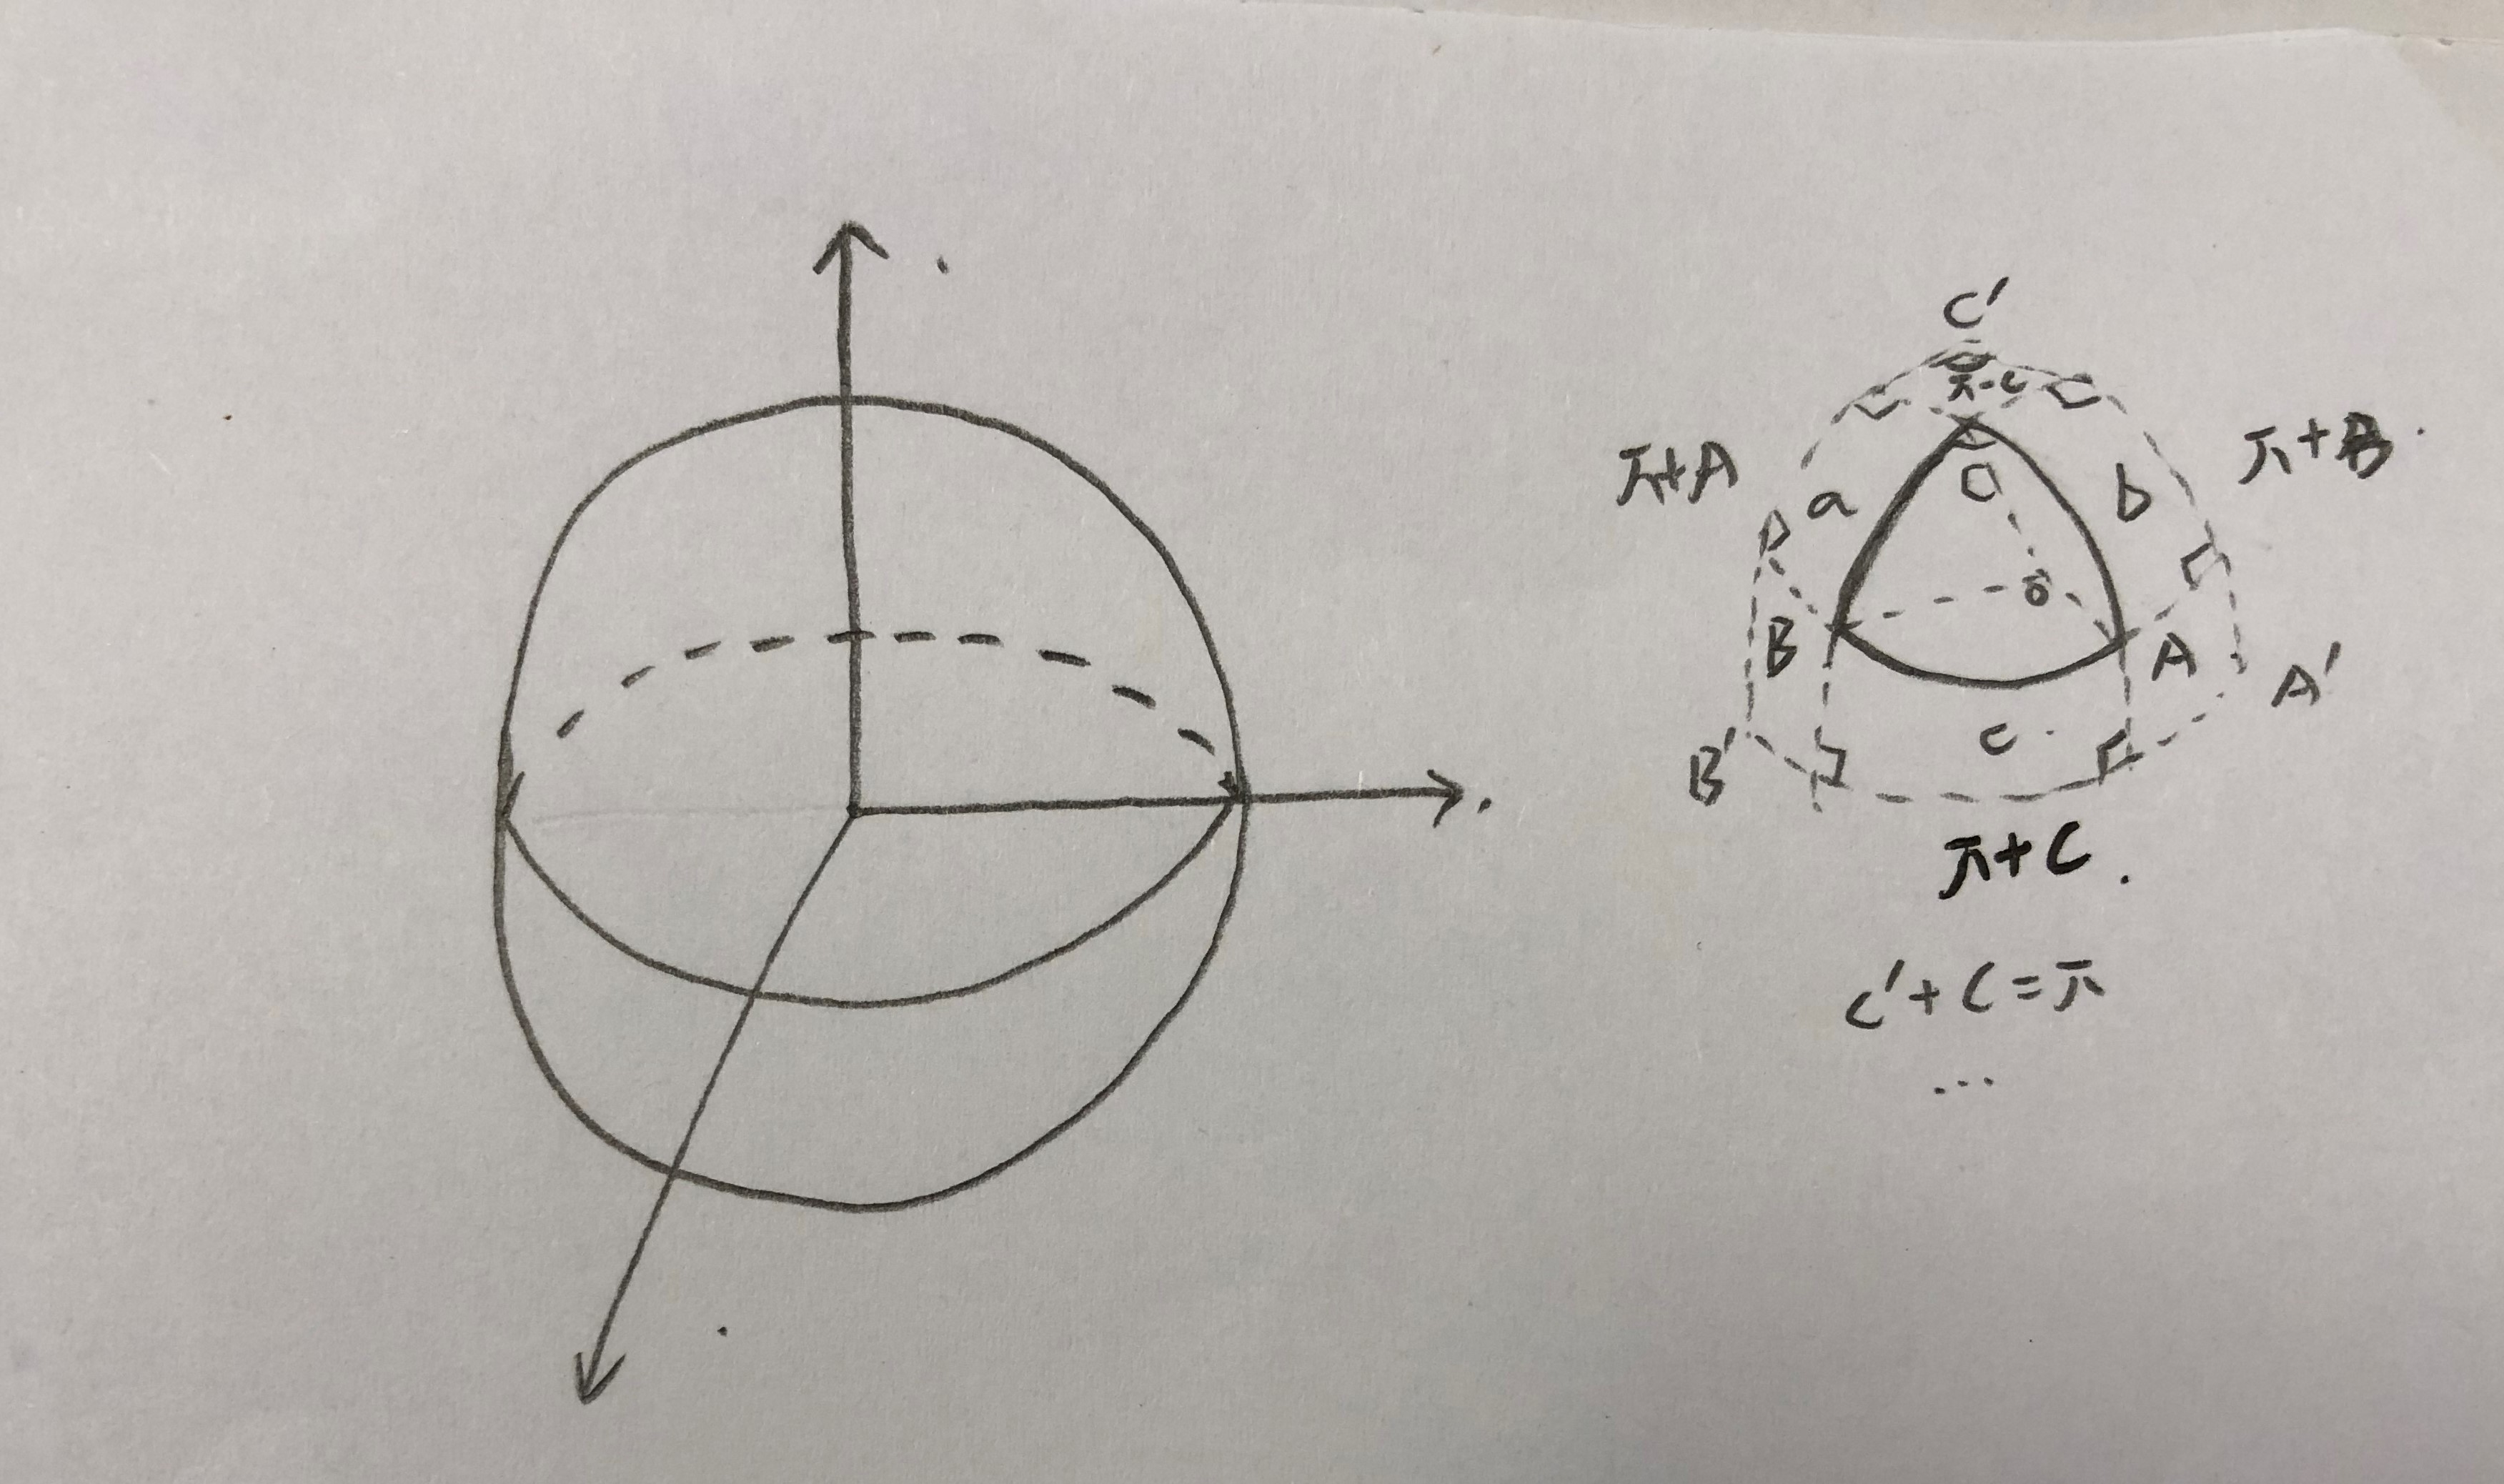
\includegraphics[width=12cm]{2.jpg}
	\caption{示意图}
	\label{fig:2}
\end{figure}
边余弦公式:$\cos{c}=\cos{a}\cos{b}+\sin{a}\sin{b}\cos{C}$

角余弦公式:$\cos{C}=-\cos{A}\cos{B}+\sin{A}\sin{B}\cos{c}$

正弦公式:$\frac{\sin{a}}{\sin{A}}=\frac{\sin{b}}{\sin{B}}=\frac{\sin{c}}{\sin{C}}$

证明:已知
\begin{gather}
	\overrightarrow{OB}\cdot\overrightarrow{OC}=\cos{a}\label{eq:1}\\
	\overrightarrow{OA}\cdot\overrightarrow{OC}=\cos{b}\label{eq:2}\\
	(\overrightarrow{OC}\times\overrightarrow{OB})\cdot(\overrightarrow{OA}\times\overrightarrow{OC})=-\sin{a}\sin{b}\cos{C}\label{eq:3}\\
	\vert(\overrightarrow{OC}\times\overrightarrow{OB})\times(\overrightarrow{OA}\times\overrightarrow{OC})\vert=\vert\sin{a}\sin{b}\sin{C}\label{eq:4}\vert
\end{gather}

由\eqref{eq:3}可证边余弦公式
\begin{equation}
	\begin{split}
		&\mathrel{\phantom{=}}(\overrightarrow{OC}\times\overrightarrow{OB})\cdot(\overrightarrow{OA}\times\overrightarrow{OC})\\
		&=[(\overrightarrow{OC}\times\overrightarrow{OB})\times\overrightarrow{OA}]\cdot\overrightarrow{OC}\\
		&=\cos{a}\cos{b}-\cos{c}=-\sin{a}\sin{b}\cos{C}
	\end{split}
\end{equation}

进而证明角余弦公式
\begin{equation}
	\cos{(\pi-C)}=\cos{(\pi-A)}\cos{(\pi-B)}-\sin{(\pi-A)}\sin{(\pi-B)}\cos{(\pi-c)}
\end{equation}

利用\eqref{eq:4}可证正弦公式
\end{document}